% Notes and solutions


% -------------------------------------------------
% Package imports
% -------------------------------------------------
\documentclass[12pt, a4paper]{article}
\usepackage[utf8]{inputenc}% Input encoding
\usepackage[english]{babel}% Set language to english
\usepackage{graphicx}% For importing graphics
\usepackage{amsthm, amsfonts, amssymb, bm}% All the AMS packages
\usepackage{mathtools}% Fixes a few AMS bugs
\usepackage[expansion=false]{microtype}% Fixes to make typography better
\usepackage{hyperref}% For \href{URL}{text}
\usepackage{fancyhdr}% For fancy headers
\usepackage[sharp]{easylist}% Easy nested lists
\usepackage{parskip}% Web-like paragraphs
\usepackage{multicol}% For multiple columns
\usepackage{tikz-cd}% For diagrams
\usepackage{microtype}
\usepackage{listings}% To include source-code
\usepackage[margin = 2.5cm, includehead]{geometry}% May be used to set margins
\usepackage{nicefrac}% Enables \nicefrac{nom}{denom}
%\usepackage[sc]{mathpazo}% A nice font, alternative to CM
\usepackage{booktabs}
\usepackage{fancyvrb} % fancy verbatim

% -------------------------------------------------
% Package setup
% -------------------------------------------------

\newcommand{\Title}{Solutions to\\``Pattern Recognition and Machine Learning''\\by Bishop}
%\newcommand{\Subtitle}{A summary of main ideas and concepts}
\newcommand{\Author}{\texttt{tommyod} @ github}
\newcommand{\listSpace}{-0.5em}% Global list space

\title{\Title}
\author{\Author}

% Shortcuts for sets and other stuff in mathematics
\newcommand{\Q}{\mathbb{Q}}
\newcommand{\R}{\mathbb{R}}
\newcommand{\C}{\mathbb{C}}
\newcommand{\D}{\mathcal{D}}
\newcommand{\F}{\mathcal{F}}
\newcommand{\Y}{\mathcal{Y}}
\newcommand{\Reg}{\mathcal{R}}
\newcommand{\Class}{\mathcal{C}}
\newcommand{\Z}{\mathbb{Z}}
\renewcommand{\sf}[1]{\mathsf{#1}}
\newcommand{\vect}[1]{\bm{#1}}
\newcommand{\norm}[1]{\left\lVert#1\right\rVert}
\newcommand{\abs}[1]{\left\lvert#1\right\rvert}

% Shortcuts for probability distributions
\DeclareMathOperator{\N}{\mathcal{N}}
\DeclareMathOperator{\Bern}{\operatorname{Bern}}
\DeclareMathOperator{\Beta}{\operatorname{Beta}}
\DeclareMathOperator{\Bin}{\operatorname{Bin}}
\DeclareMathOperator{\St}{\operatorname{St}}
\DeclareMathOperator{\U}{\operatorname{U}}
\DeclareMathOperator{\KL}{\operatorname{KL}}

% Shortcuts for statistical operators
\DeclareMathOperator{\E}{\mathbb{E}}
\DeclareMathOperator{\var}{\operatorname{var}}
\DeclareMathOperator{\cov}{\operatorname{cov}}
\DeclareMathOperator{\SD}{\operatorname{SD}}
\renewcommand{\H}{\operatorname{H}}



% Change the section command to inluce lines, save space, etc.
%\usepackage{titlesec}
%\titlespacing\subsection{0pt}{6pt plus 4pt minus 2pt}{-0.8em plus 4pt minus 2pt}
%\titlespacing\paragraph{0pt}{6pt plus 4pt minus 2pt}{8pt plus 4pt minus 2pt}
%\titleformat{\section}
%{\normalfont\Large\bfseries}{\thesection}{0em}{$\vartriangleright$ }[{\titlerule[1.2pt]}]

% -------------------------------------------------
% Document start
% -------------------------------------------------
\begin{document}
	
\maketitle
\begin{abstract}
This document contains some notes and solutions to the book TODO.fødselsnrfødselsnr

\begin{figure}[ht!]
	\centering
	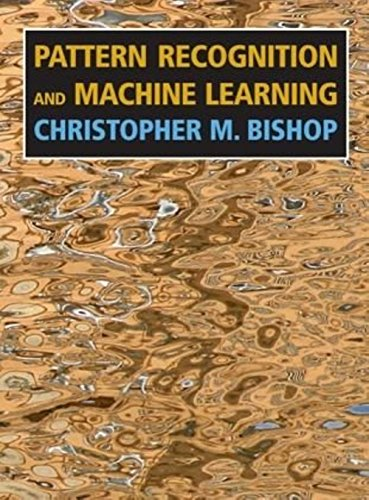
\includegraphics[width=0.25\linewidth]{figs/bishop}
	\caption{The front cover of \cite{bishop_pattern_2011}.}
	\label{fig:duda}
\end{figure}
\end{abstract}

\clearpage

{\small \tableofcontents}


\clearpage
\section{Chapter notes}

% ----------------------------------------------------------------------------
\subsection{Introduction}
\begin{easylist}[itemize]
	\ListProperties(Space=\listSpace, Space*=\listSpace, Numbers1=l, FinalMark1={)})
	# sdf
\end{easylist}

% ----------------------------------------------------------------------------
\subsection{Probability Distributions}
\begin{easylist}[itemize]
	\ListProperties(Space=\listSpace, Space*=\listSpace, Numbers1=l, FinalMark1={)})
	# sdf
\end{easylist}

% ----------------------------------------------------------------------------
\subsection{Linear Models for Regression}
\begin{easylist}[itemize]
	\ListProperties(Space=\listSpace, Space*=\listSpace, Numbers1=l, FinalMark1={)})
	# sdf
\end{easylist}

% ----------------------------------------------------------------------------
\subsection{Linear Models for Classification}
\begin{easylist}[itemize]
	\ListProperties(Space=\listSpace, Space*=\listSpace, Numbers1=l, FinalMark1={)})
	# sdf
\end{easylist}

% ----------------------------------------------------------------------------
\subsection{Neural networks}
\begin{easylist}[itemize]
	\ListProperties(Space=\listSpace, Space*=\listSpace, Numbers1=l, FinalMark1={)})
	# sdf
\end{easylist}

% ----------------------------------------------------------------------------
\subsection{Kernel methods}
\begin{easylist}[itemize]
	\ListProperties(Space=\listSpace, Space*=\listSpace, Numbers1=l, FinalMark1={)})
	# sdf
\end{easylist}

% ----------------------------------------------------------------------------
\subsection{Sparse Kernel Machines}
\begin{easylist}[itemize]
	\ListProperties(Space=\listSpace, Space*=\listSpace, Numbers1=l, FinalMark1={)})
	# sdf
\end{easylist}

% ----------------------------------------------------------------------------
\subsection{Graphical Models}
\begin{easylist}[itemize]
	\ListProperties(Space=\listSpace, Space*=\listSpace, Numbers1=l, FinalMark1={)})
	# sdf
\end{easylist}

% ----------------------------------------------------------------------------
\subsection{Mixture Models and EM}
\begin{easylist}[itemize]
	\ListProperties(Space=\listSpace, Space*=\listSpace, Numbers1=l, FinalMark1={)})
	# sdf
\end{easylist}

% ----------------------------------------------------------------------------
\subsection{Approximate Interference}
\begin{easylist}[itemize]
	\ListProperties(Space=\listSpace, Space*=\listSpace, Numbers1=l, FinalMark1={)})
	# sdf
\end{easylist}

% ----------------------------------------------------------------------------
\subsection{Sampling Methods}
\begin{easylist}[itemize]
	\ListProperties(Space=\listSpace, Space*=\listSpace, Numbers1=l, FinalMark1={)})
	# sdf
\end{easylist}

% ----------------------------------------------------------------------------
\subsection{Continuous Latent Variables}
\begin{easylist}[itemize]
	\ListProperties(Space=\listSpace, Space*=\listSpace, Numbers1=l, FinalMark1={)})
	# sdf
\end{easylist}

% ----------------------------------------------------------------------------
\subsection{Sequential Data}
\begin{easylist}[itemize]
	\ListProperties(Space=\listSpace, Space*=\listSpace, Numbers1=l, FinalMark1={)})
	# sdf
\end{easylist}

% ----------------------------------------------------------------------------
\subsection{Combining Models}
\begin{easylist}[itemize]
	\ListProperties(Space=\listSpace, Space*=\listSpace, Numbers1=l, FinalMark1={)})
	# sdf
\end{easylist}

% ----------------------------------------------------------------------------





\clearpage

\section{Chapter summaries}

% ----------------------------------------------------------------------------
\subsection{Introduction}
\begin{easylist}[itemize]
	\ListProperties(Space=\listSpace, Space*=\listSpace, Numbers1=l, FinalMark1={)})
	# sdf
\end{easylist}

% ----------------------------------------------------------------------------
\subsection{Probability Distributions}
\begin{easylist}[itemize]
	\ListProperties(Space=\listSpace, Space*=\listSpace, Numbers1=l, FinalMark1={)})
	# sdf
\end{easylist}

% ----------------------------------------------------------------------------
\subsection{Linear Models for Regression}
\begin{easylist}[itemize]
	\ListProperties(Space=\listSpace, Space*=\listSpace, Numbers1=l, FinalMark1={)})
	# sdf
\end{easylist}

% ----------------------------------------------------------------------------
\subsection{Linear Models for Classification}
\begin{easylist}[itemize]
	\ListProperties(Space=\listSpace, Space*=\listSpace, Numbers1=l, FinalMark1={)})
	# sdf
\end{easylist}

% ----------------------------------------------------------------------------
\subsection{Neural networks}
\begin{easylist}[itemize]
	\ListProperties(Space=\listSpace, Space*=\listSpace, Numbers1=l, FinalMark1={)})
	# sdf
\end{easylist}

% ----------------------------------------------------------------------------
\subsection{Kernel methods}
\begin{easylist}[itemize]
	\ListProperties(Space=\listSpace, Space*=\listSpace, Numbers1=l, FinalMark1={)})
	# sdf
\end{easylist}

% ----------------------------------------------------------------------------
\subsection{Sparse Kernel Machines}
\begin{easylist}[itemize]
	\ListProperties(Space=\listSpace, Space*=\listSpace, Numbers1=l, FinalMark1={)})
	# sdf
\end{easylist}

% ----------------------------------------------------------------------------
\subsection{Graphical Models}
\begin{easylist}[itemize]
	\ListProperties(Space=\listSpace, Space*=\listSpace, Numbers1=l, FinalMark1={)})
	# sdf
\end{easylist}

% ----------------------------------------------------------------------------
\subsection{Mixture Models and EM}
\begin{easylist}[itemize]
	\ListProperties(Space=\listSpace, Space*=\listSpace, Numbers1=l, FinalMark1={)})
	# sdf
\end{easylist}

% ----------------------------------------------------------------------------
\subsection{Approximate Interference}
\begin{easylist}[itemize]
	\ListProperties(Space=\listSpace, Space*=\listSpace, Numbers1=l, FinalMark1={)})
	# sdf
\end{easylist}

% ----------------------------------------------------------------------------
\subsection{Sampling Methods}
\begin{easylist}[itemize]
	\ListProperties(Space=\listSpace, Space*=\listSpace, Numbers1=l, FinalMark1={)})
	# sdf
\end{easylist}

% ----------------------------------------------------------------------------
\subsection{Continuous Latent Variables}
\begin{easylist}[itemize]
	\ListProperties(Space=\listSpace, Space*=\listSpace, Numbers1=l, FinalMark1={)})
	# sdf
\end{easylist}

% ----------------------------------------------------------------------------
\subsection{Sequential Data}
\begin{easylist}[itemize]
	\ListProperties(Space=\listSpace, Space*=\listSpace, Numbers1=l, FinalMark1={)})
	# sdf
\end{easylist}

% ----------------------------------------------------------------------------
\subsection{Combining Models}
\begin{easylist}[itemize]
	\ListProperties(Space=\listSpace, Space*=\listSpace, Numbers1=l, FinalMark1={)})
	# sdf
\end{easylist}

% ----------------------------------------------------------------------------
















\clearpage
\section{Exercises}

% ----------------------------------------------------------------------------
\subsection{Introduction}
\subsubsection*{Exercise 1.2}
We start with Equation (1.4) and differentiate it with respect to $w_i$:
\begin{align*}
	\partial_{w_i} \tilde{E}(\vect{w})
	&= \sum_{n=1}^{N} \left[ y(x_n, \vect{w}) - t_n \right] \partial_{w_i} y(x_n, \vect{w}) + \lambda w_i \\
	&= \sum_{n=1}^{N} \left[ y(x_n, \vect{w}) - t_n \right] (x_n)^i + \lambda w_i \\
	&= \sum_{n=1}^{N} \left[ \sum_{j=0}^{M} w_j (x_n)^j - t_n \right] (x_n)^i + \lambda w_i = 0
\end{align*}
Multiplying through the $(x_n)^i$ and rearranging terms yields
\begin{equation*}
	\sum_{j=0}^{M} w_j \underbrace{\sum_{n=1}^{N} (x_n)^{i+j}}_{A_{ij}}
	+
	\lambda w_i = \underbrace{\sum_{n=1}^{N}  (x_n)^i t_n}_{T_{ij}},
\end{equation*}
where the definitions of $A_{ij}$ and $T_{ij}$ are identical to those given in Exercise 1.1.
Finally we employ the kronecker delta symbol $\delta_{ij}$ to pull the $w_i$ into the sum, since $\lambda w_j = \sum_{j=0}^{N} \lambda \delta_{ij} w_i$ we have
\begin{equation*}
	\sum_{j=0}^{M}  \left( A_{ij} + \delta_{ij} \lambda \right) w_j
	 = T_{ij}.
\end{equation*}
This solves the problem.
Notice that in vector notation this system can be written as 
\begin{equation*}
	\left( \vect{\Phi}^T \vect{\Phi} + \vect{I}\lambda \right) \vect{w} = \vect{\Phi}^T \vect{t},
\end{equation*}
where $\vect{\Phi}_{ij}= (x_i)^j$.
Solving the system solves the regularized polynomial fitting problem.


\subsubsection*{Exercise 1.8}
We first show that the expected value is $\mu$.
We define $K(\sigma) = 1 / \sqrt{2 \pi} \sigma$ and evaluate the integral
\begin{align*}
	\E \left[x\right] &= \int K(\sigma) \exp \left( - \frac{1}{2 \sigma^2} \left(x - \mu \right)^2 \right) x \, dx \\
	&= \int K(\sigma) \exp \left( - \frac{1}{2 \sigma^2} z^2 \right) (z + \mu) \, dz \tag{change of variables}\\
	&= \int K(\sigma) \exp \left( - \frac{1}{2 \sigma^2} z^2 \right) z \, dz 
	+
	 \mu \int K(\sigma) \exp \left( - \frac{1}{2 \sigma^2} z^2 \right) \, dz \\
	 & = 0 + \mu,
\end{align*}
where the first integral in the second to last line is zero because it's an odd function integrated over the real line, and the second integral evaluates to $\mu$ since the integrand is unity (it's a centered normal distribution, which has integral $1$).

The second part of the problem asks us to verify that $\E \left[ x^2 \right] = \mu^2 + \sigma^2$.
We factor the normal distribution as $\N\left( x \mid \mu, \sigma^2\right) = K(\sigma^2) E(\sigma^2)$, where
\begin{alignat*}{3}
	& K(\sigma^2) = \left( 2 \pi \sigma^2 \right)^{-1/2} 
	&& \qquad \frac{\partial K}{\partial \sigma^2} = - \left( 2 \pi \sigma^2 \right)^{-3/2} \pi = -K(\sigma^2)^3 \pi \\
	& E(\sigma^2) = \exp \left( - \frac{1}{2 \sigma^2} \left( x - \mu \right)^2 \right)
	&& \qquad \frac{\partial E}{\partial \sigma^2} = \frac{1}{2\sigma^4} \left( x - \mu\right)^2 E(\sigma^2).
\end{alignat*}
This allows us to use the product rule of calculus, we have
\begin{gather*}
	\frac{\partial}{\partial \sigma^2} \left( \int K(\sigma^2) E(\sigma^2) \, dx = 1 \right) \\
	\int K' E + K E' \, dx = 0 \\
	\int KE \left( -\pi K^2 + \frac{1}{2 \sigma^4} (x - \mu)^2 \right) \, dx = 0.
\end{gather*}
Substituting $- \pi K^2 = - 1 / (2 \sigma^2)$, expanding the square term, multiplying out the $KE$ term and performing the integrals, we obtain
\begin{equation*}
	-\frac{1}{2\sigma^2} + \frac{1}{2 \sigma^4} \int KE x^2 \, dx + 0 - \frac{\mu^2}{2 \sigma^4} = 0,
\end{equation*}
and solving this for the unknown integral yields $\operatorname{E}\left[x^2\right] = \int KE x^2 \, dx = \mu^2 + \sigma^2$.

To show that equation (1.51) holds, notice that
\begin{align*}
	\var \left[ x \right] &= \E\left[ (x - \E\left[x\right])^2\right] \\
	&= \E\left[ x^2 - 2 x \mu + \mu ^2\right] \\
	&= \E\left[ x^2\right] - 2 \mu^2 + \mu^2 \\
	&= \E\left[ x^2\right] - \E\left[ x\right],
\end{align*}
where we have used $\mu$ interchangeably with $\E\left[ x\right]$. 



\subsubsection*{Exercise 1.10}
Recall that the definition of the expected value is
$\E\left[x\right] = \int p(x) x \, dx$, and that $\int p(x) \, dx = 1$. 
Statistical independence means that $p(x, y)$ factors as $p(x)p(y)$, so we have
\begin{align*}
	\E\left[x + y\right] &= \iint p(x, y) (x+y) \, dx \, dy \\
	&= \iint p(x) p(y) (x+y) \, dx \, dy \tag{independence} \\
	&= \iint p(x) p(y) x \, dx \, dy + \iint p(x) p(y) y \, dx \, dy \\
	&= \int p(y) \left( \int  p(x)  x \, dx \right) \, dy + \int p(y) y \left( \int p(x)  \, dx \right) \, dy \\
	&= \int p(y) \left( \E \left[ x \right] \right) \, dy + \int p(y) y \left( 1 \right) \, dy \tag{by definition} \\
	&= \E\left[x\right] + \E\left[y\right]
\end{align*}
To show that $\var\left[x + y\right] = \var\left[x\right] + \var\left[y\right]$, we use the preceding result along with the definition from equation (1.38) in \cite{bishop_pattern_2011}  $\var\left[x\right] = \E\left[ (x - \E\left[x\right])^2\right]$ to write
\begin{align*}
	\var\left[x + y\right] &= \E\left[ \left( (x + y) - \E \left[ x + y \right] \right)^2\right] \\
	&= \E\left[ \left( \left(x - \E\left[x\right]\right) + \left(y - \E\left[y\right]\right) \right)^2\right] \tag{rearranging} \\
	&= \E\left[  \left(x - \E\left[x\right]\right)^2 + 2 \left(x - \E\left[x\right]\right) \left(y - \E\left[y\right]\right) + \left(y - \E\left[y\right]\right)^2\right] \\
	&= \E\left[  \left(x - \E\left[x\right]\right)^2 \right]
	+
	\underbrace{\E\left[   2 \left(x - \E\left[x\right]\right) \left(y - \E\left[y\right]\right) \right]}_{0}
	+
	\E\left[   \left(y - \E\left[y\right]\right)^2\right] \\
	&= \var\left[x\right] + \var\left[y\right].
\end{align*}
The cross term vanishes since $x$ and $y$ are independent.
We will not show this in detail, but it can be shown by first noticing that $\E \left[xy\right] = \E \left[x\right] \E \left[y\right]$ when $x$ and $y$ are independent, and then showing that $\E\left[    \left(x - \E\left[x\right]\right) \right] = \E\left[ x \right] - \E\left[ x \right] = 0$.

\subsubsection*{Exercise 1.15}
TODO


\subsubsection*{Exercise 1.21}
Starting with $a \leq b$, we multiply both sides by $a > 0$ to obtain $a^2 \leq ab$.
We can take the square root of both sides and preserve the inequality, since the square root is monotonically increasing.
Doing so, we obtain the desired inequality.

To prove the inequality, we apply the inequality on each term in equation (1.78), then replace the integral over $\mathcal{R}_1 \cup \mathcal{R}_2$ with the real line.
\begin{align*}
	p(\text{mistake}) &= \int_{\mathcal{R}_1} p(\vect{x}, \mathcal{C}_1) \, d \vect{x}
	+
	\int_{\mathcal{R}_2} p(\vect{x}, \mathcal{C}_2) \, d \vect{x} \\
	&\leq 
	 \int_{\mathcal{R}_1} \left\{ p(\vect{x}, \mathcal{C}_1) p(\vect{x}, \mathcal{C}_2) \right\}^{1/2} \, d \vect{x}
	+
	\int_{\mathcal{R}_2} \left\{ p(\vect{x}, \mathcal{C}_2) p(\vect{x}, \mathcal{C}_1) \right\}^{1/2} \, d \vect{x} \\
	&= \int \left\{ p(\vect{x}, \mathcal{C}_2) p(\vect{x}, \mathcal{C}_1) \right\}^{1/2} \, d \vect{x}
\end{align*}

% ----------------------------------------------------------------------------
\subsection{Probability Distributions}
\subsubsection*{Problem X.Y}
\begin{easylist}[enumerate]
	\ListProperties(Space=\listSpace, Space*=\listSpace, Numbers1=l, FinalMark1={)})
	# sdf
\end{easylist}

% ----------------------------------------------------------------------------
\subsection{Linear Models for Regression}
\subsubsection*{Problem X.Y}
\begin{easylist}[enumerate]
	\ListProperties(Space=\listSpace, Space*=\listSpace, Numbers1=l, FinalMark1={)})
	# sdf
\end{easylist}

% ----------------------------------------------------------------------------
\subsection{Linear Models for Classification}
\subsubsection*{Problem X.Y}
\begin{easylist}[enumerate]
	\ListProperties(Space=\listSpace, Space*=\listSpace, Numbers1=l, FinalMark1={)})
	# sdf
\end{easylist}

% ----------------------------------------------------------------------------
\subsection{Neural networks}
\subsubsection*{Problem X.Y}
\begin{easylist}[enumerate]
	\ListProperties(Space=\listSpace, Space*=\listSpace, Numbers1=l, FinalMark1={)})
	# sdf
\end{easylist}

% ----------------------------------------------------------------------------
\subsection{Kernel methods}
\subsubsection*{Problem X.Y}
\begin{easylist}[enumerate]
	\ListProperties(Space=\listSpace, Space*=\listSpace, Numbers1=l, FinalMark1={)})
	# sdf
\end{easylist}

% ----------------------------------------------------------------------------
\subsection{Sparse Kernel Machines}
\subsubsection*{Problem X.Y}
\begin{easylist}[enumerate]
	\ListProperties(Space=\listSpace, Space*=\listSpace, Numbers1=l, FinalMark1={)})
	# sdf
\end{easylist}

% ----------------------------------------------------------------------------
\subsection{Graphical Models}
\subsubsection*{Problem X.Y}
\begin{easylist}[enumerate]
	\ListProperties(Space=\listSpace, Space*=\listSpace, Numbers1=l, FinalMark1={)})
	# sdf
\end{easylist}

% ----------------------------------------------------------------------------
\subsection{Mixture Models and EM}
\subsubsection*{Problem X.Y}
\begin{easylist}[enumerate]
	\ListProperties(Space=\listSpace, Space*=\listSpace, Numbers1=l, FinalMark1={)})
	# sdf
\end{easylist}

% ----------------------------------------------------------------------------
\subsection{Approximate Interference}
\subsubsection*{Problem X.Y}
\begin{easylist}[enumerate]
	\ListProperties(Space=\listSpace, Space*=\listSpace, Numbers1=l, FinalMark1={)})
	# sdf
\end{easylist}

% ----------------------------------------------------------------------------
\subsection{Sampling Methods}
\subsubsection*{Problem X.Y}
\begin{easylist}[enumerate]
	\ListProperties(Space=\listSpace, Space*=\listSpace, Numbers1=l, FinalMark1={)})
	# sdf
\end{easylist}

% ----------------------------------------------------------------------------
\subsection{Continuous Latent Variables}
\subsubsection*{Problem X.Y}
\begin{easylist}[enumerate]
	\ListProperties(Space=\listSpace, Space*=\listSpace, Numbers1=l, FinalMark1={)})
	# sdf
\end{easylist}

% ----------------------------------------------------------------------------
\subsection{Sequential Data}
\subsubsection*{Problem X.Y}
\begin{easylist}[enumerate]
	\ListProperties(Space=\listSpace, Space*=\listSpace, Numbers1=l, FinalMark1={)})
	# sdf
\end{easylist}

% ----------------------------------------------------------------------------
\subsection{Combining Models}
\subsubsection*{Problem X.Y}
\begin{easylist}[enumerate]
	\ListProperties(Space=\listSpace, Space*=\listSpace, Numbers1=l, FinalMark1={)})
	# sdf
\end{easylist}

% ----------------------------------------------------------------------------



































\bibliographystyle{apalike}%alpha, apalike is also good
\bibliography{../bibliography}


\end{document}
